%%%%%%%% ICML 2021 EXAMPLE LATEX SUBMISSION FILE %%%%%%%%%%%%%%%%%
\documentclass{article}
\usepackage{algorithm2e}
\usepackage{algorithmic}
\usepackage{algorithm}
% Recommended, but optional, packages for hs and better typesetting:
\usepackage{microtype}
\usepackage{graphicx}
\usepackage{amsmath}
\usepackage{amsfonts}
\usepackage{appendix}
\usepackage{subfigure}
\usepackage{booktabs} % for professional tables
\usepackage{hyperref}
% Attempt to make hyperref and algorithmic work together better:
\newcommand{\theHalgorithm}{\arabic{algorithm}}
\usepackage{icml2021}
\usepackage{float}
\usepackage{enumitem}

\begin{document}
\twocolumn[
\icmltitle{Reinforcement Learning 2024
Assignment 3: Policy-based Reinforcement Learning}

\icmlsetsymbol{equal}{*}
\begin{icmlauthorlist}
\icmlauthor{Sherry Usman}{equal,to}
\icmlauthor{Qin Zhipei}{equal,to}
\icmlauthor{Megan Mirnalini Sundaram R}{equal,to}
\end{icmlauthorlist}

\icmlaffiliation{to}{Leiden University}

% You may provide any keywords that you
% find helpful for describing your paper; these are used to populate
% the "keywords" metadata in the PDF but will not be shown in the document
\icmlkeywords{Machine Learning, Deep Q-Learning, Experience Replay, Target Network}

\vskip 0.3in
]

\begin{abstract}
This paper explores policy-based reinforcement learning in detail and the commonly used algorithms in policy-based learning. We explore this in one of the OpenAI Gym Libraries - Lunar Lander. We implement algorithms such as REINFORCE, Actor-Critic and their specifications and also delve further into the effects of bootstrapping and baseline subtraction on actor-critic networks. We compare and contrast the performances of the algorithms with variations in learning rate, hidden layers and number of neurons. We also analyze the effects of entropy regularization on these algorithms and compare the performances of the algorithms with and without entropy regularization. 
\end{abstract}

\section {Introduction}
In this paper we will delve into the Lunar Lander environment taken from the OpenAI Gym library. The Lunar Lander game is a classical reinforcement learning environment, based on the physics enginge box2d \cite{brockman2016openai} where the goal is to optimise the trajectory of a rocket such that it lands between the two flags.
 While a number of different techniques can be used to solve this problem, our paper specifically concentrates on the use of  \textbf{REINFORCE} and \textbf{Actor-Critic}. Through this paper, we hope to provide the specifications of various Policy Gradient methods while also including the tried and tested hyper-parameters that produce the best results.%$$ best exploration-to-exploitation ratio. \newline

\begin{figure}[htbp]
\centering
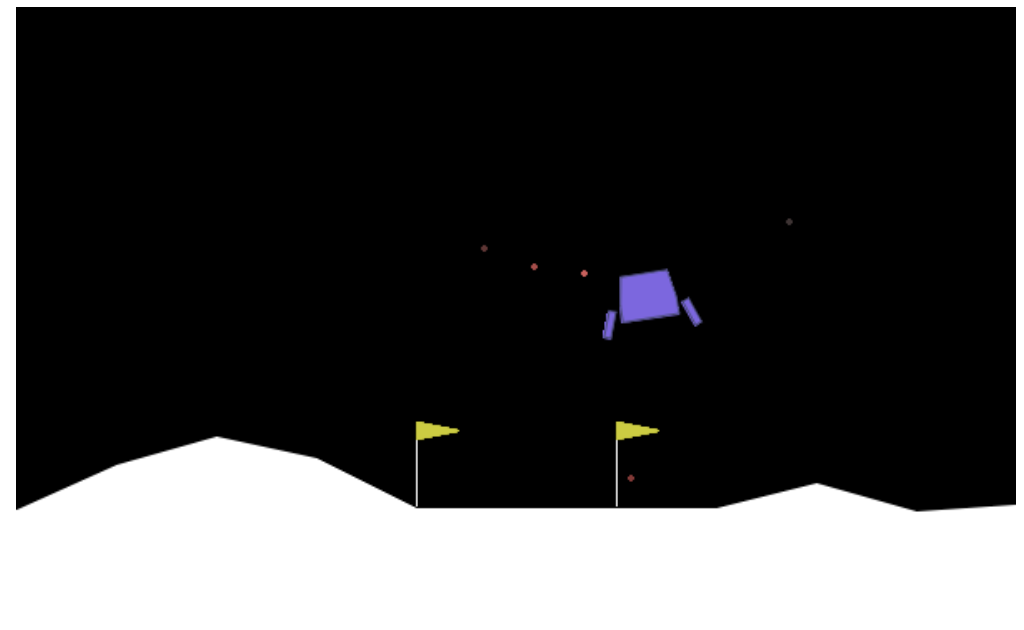
\includegraphics[width=0.7\linewidth]{Report/images/01.visualisation.png}
\caption{\label{fig:Visualization of the Cart-pole} A visualisation of the Lunar Lander problem}
\end{figure}

%\label{Introduction and General Strategy}

The Lunar Lander environment poses a number of unique challenges compared to the environments we have encountered previously. As shown in \emph{Table 1}, while the action space $A$ is still discrete with four potential actions, the observation space is an 8-dimensional vector comprising of the positional coordinates of the lunar lander (x and y), its linear velocities in x and in y respectively, its angle, its angular velocities and two boolean values that represent whether each leg is in contact with the ground or not. The inclusion of a continuous action or state space makes tabular/value-based reinforcement learning algorithms quickly unfeasible as the cost of storing the values for each state-action pair makes our problem much more complex. 
\par Thus, to tackle this problem we use Policy Gradient methods which can handle continuous state and action spaces much better, as they directly optimise the expected return and can provide continuous action distributions as output, making them also suitable for continuous action spaces.

\begin{table}[htbp]
\centering
\begin{tabular}{|l|c|}
\hline
\textbf{Value} & \textbf{Action} \\
\hline
0  & Do nothing \\
\hline
1 & fire left orientation engine \\
\hline
2  & fire main engine \\
\hline
3 & fire right orientation engine  \\
\hline
\end{tabular}
\caption{Action Space of Lunar Lander Environment}
\label{tab:hyper-parameters}
\end{table}



\section{Framework}
For our implementation of Policy Gradient Methods, we used the Python \textbf{Pytorch} package. 
\par Our initial structure is as follows: an input layer of size 8 corresponding to the size of the observation space. This input layer feeds into a first hidden layer with 128 nodes. This then feeds into a hidden layer comprising of 128 nodes which finally outputs to a layer comprising of 1 node representing the action that should be taken. Since the Lunar Lander environment is also highly stochastic, to reduce noise in our graphs we computed different algorithms over 1000 episodes and averaged the results every 5 episodes to capture the general trends. 
\par Furthermore, we are aware that total rewards is not always the best parameter to measure algorithm accuracy as the number of timesteps in each episode may differ and lead to exploding or shrinking rewards. Thus, in some cases we also include another parameter to measure accuracy which is the number of timesteps.

%In this section we experiment with various hyper-parameters such as batch size, learning rates and more while also fine-tuning our neural network by modifying the number of hidden layers and neurons in each layer.% Since this environment is also highly stochastic, we de-noise by testing over 1000 episodes and averaging our results over every 10 episodes.
%For 

\section{Policy-Based Reinforcement Learning}
\par The policies we looked at in the previous papers were \emph{value-based}. This means that they looked at state-value pairs in the environment and calculated the rewards of such pairs using different exploration strategies like Boltzmann or Epsilon-Greedy. Policy based reinforcement learning methods differ from value-based method as they do not utilize a value function to determine the next possible action. Used primarily in  continuous action space RL environments, policy based reinforcement learning methods use a parameterized policy function $\pi_\theta$ where $\theta$ represents the parameters of the function. 
\par During training the agent iteratively interacts with the environment and after a number of episodes the collected data known as the trajectory $\tau$ is evaluated to understand the performance of the policy. 
\begin{itemize}[itemsep=0pt]
    \item If $\tau$ yields high rewards then the parameters $\theta$ are adjusted in such a way that the likelihood of taking similar actions as those in $\tau$ is increased.
    \item On the other hand if the trajectory $\tau$ yields lower rewards then $\theta$ is adjusted in such a way that the likelihood of taking similar actions as those in $\tau$ is decreased.
\end{itemize}  
This process of iteratively evaluating the trajectories and updating the parameters according to the obtained rewards/losses helps to refine the policy to maximize cumulative rewards in the long run \cite{plaat-deeprl}.
\par Policy Gradient methods pose a number of advantages that make them suitable algorithms for reinforcement learning environments. Firstly since Policy Gradient methods directly optimise a policy function rather than approximating the value of each state-action pair they tend to be much more stable and robust in high-dimensional environments like Lunar Lander, allowing more stable convergence after a number of training episodes. Additionally, since they do not need state-action pairs to approximate values they do not run the risk of getting stuck in local optima like value-based methods and can approximate complex non-linear relationships more accurately than value-based algorithms. Lastly, policy gradient methods tend to be more sample efficient as they need less existing data to achieve a good performance and can even approximate rewards in areas with sparse reward signals. 

\par
There are a number of different policy-based reinforcement learning algorithms. However for this paper, we are limiting the scope of our research to the algorithms listed below: 

\begin{itemize}[itemsep=0.0pt]
\item REINFORCE
\item Actor-Critic with Bootstrapping
\item Actor-Critic with Baseline Subtraction
\item Actor Critic with Bootstrapping and Baseline Subtraction
\end{itemize}
These algorithms are discussed in the future sections. 

\par For any reinforcement learning algorithm it is necessary to decide on an action selection policy. Traditional action selection algorithms used before such as Boltzmann or E-greedy cannot be used in this paper as they are better suited for value-based reinforcement learning algorithms working with a discrete action space and/or state space. This is because both epsilon-greedy and Boltzman are algorithms that scans potential actions that can be taken by the agent at a particular state and calculates their value, which helps inform the agent's next step. This is not possible in Policy Gradient methods which are less concerned with state-action pairs and more with the policy function. 
\par Hence, in this paper we work with \textbf{Entropy Regularisation}. Entropy regularisation is an exploration technique that helps balance the exploration to exploitation ratio by encouraging the agent to explore more diverse actions and unfamiliar spaces. It does this by increasing by adding an entropy term to the loss function to promote action diversity and preventing sub-optimising to local rewards. The entropy term $H(X)$ is defined in the equation below. %

\begin{equation*}
H(X) = - \sum \pi(x) log(\pi(x)) %t + 1] 
\end{equation*}
where
\begin{itemize}[itemsep=0.0pt]
\renewcommand\labelitemi{.}
\item x is the set of possible actions
\item $\pi(x)$ is a function representing the probability of taking an action x
%\item H(X) is the entropy of the action distribution capturing the randomness of taking an action x
\end{itemize}
\subsection{REINFORCE}
\par REINFORCE is a commonly used Policy-based Reinforcement Learning algorithm which is also termed as a classic Monte-Carlo Policy Gradient algorithm. \cite{sutton-barlo}. It was first introduced in 1992 by Ronald J. Williams with an aim to maximise expected cumulative rewards by adjusting the policy parameters. It does this by learning from the agent trajectory (including the visited states, executed actions and incurred rewards) and estimating gradients. Because it needs a full trajectory in order to construct a sample space it is updated as an off-policy algorithm. 
\begin{equation}
\pi_\theta(a, s) = Pr(A_t = a | St = s, \theta_t = \theta)
\end{equation}
The equation above helps us recall the policy function $\pi_{\theta}(a, s)$ which indicates the probability of taking an action a in the state s with the parameters $\theta$.
We can also define a trajectory $\tau$ as the sum of rewards when following a particular path. This is shown in the equation below.
\begin{equation}
R(\tau) = [\sum_{t=0}^{T-1}r_t] 
\end{equation}

\par The REINFORCE algorithm optimises the policy function $\pi_{\theta}(a,s)$ by fine-tuning its parameters $\theta$ such that it increases the likelihood of actions in trajectories $\tau$ which lead to higher cumulative rewards. It does this by calculating the total expected rewards J($\theta$) with respect to a particular parameter value $\theta$ and adjusting $\theta$ accordingly. Thus, J($\theta$) is optimised as shown in equation 2.
\begin{equation}
\nabla J(\theta) = E_{\pi_\theta}[ R(\tau)] =   E_{\pi_\theta} (\sum_{t=0}^{T-1} \nabla log\pi_\theta(a_t s_t) R(\tau)]
\end{equation}

where $\nabla J(\theta)$ represents the gradient in the expected return function J($\theta$), E$\pi_\theta$ denotes the expectation over trajectories R sampled under policy $\pi_\theta$, $R_{\tau}$ indicates the rewards obtained from the trajectory $\tau$ and $\pi_\theta$ indicates the policy function with parameters $\theta$.  \newline
%Thus $\theta$ is optimised to be equal to the gradient ascent of the partial derivative with respect to $\theta$ of $J(\theta)$. The equation for optimisation is shown below.
%\begin{equation}
%\theta = \theta + \frac{\mathrm{d}  }{\mathrm{d} \theta} J(\theta)
%\end{equation}
%Based on this, the expected cumulative rewards is updated.

The algorithm for REINFORCE can thus be defined as follows. 
\begin{algorithm}[h!]
\caption{REINFORCE Algorithm}
\SetAlgoLined
\DontPrintSemicolon
\small % Set font size to small
\KwData{parameter $\theta$, policy function $\pi_\theta$, maximum time-steps $T$, number of episodes $E$, learning_rate $\alpha$}
\KwResult{Selected action}
Initialise $\theta$ arbitrarily\;\\
\For{$e = 1$ \KwTo $E$}{
    Initialise state $s$\;
    \For{$t = 1$ \KwTo $T-1$}
    {
     \item Sample action $a$ from $\pi_\theta$\;
     \item Execute action $a$ and get the next state $s_{t+1}$ and  reward $r_t$\; 
     \item $\theta \leftarrow \theta + \alpha \cdot \nabla_\theta \log \pi_\theta(a_t | s_t) R(\tau)$;
    }
}
Return parameter $\theta$\;
\end{algorithm}

\begin{figure}[h!]
\centering
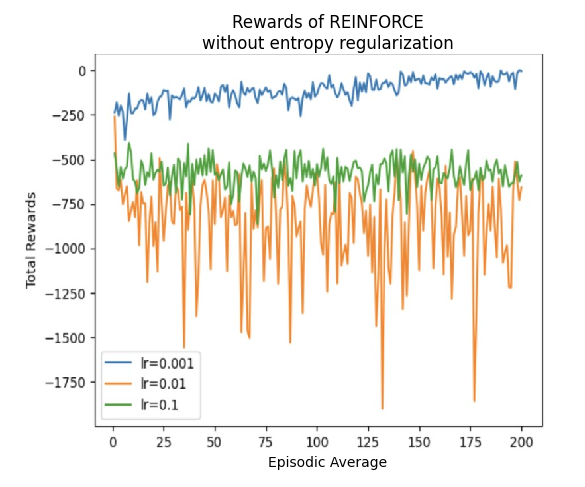
\includegraphics[width=0.85\linewidth]{Report/images/02.Rewards_of_REINFORCE_without_ER.png}
\caption{\label{fig:Reinforce Rewards}The figure above shows the rewards of REINFORCE without entropy regularisation with different learning rates. As we can see, almost all of learning rates show a rising trend of rewards, with the graph for learning rates 0.01 and 0.001 showing the most promise. }
\end{figure}


\begin{figure}[h!]
\centering
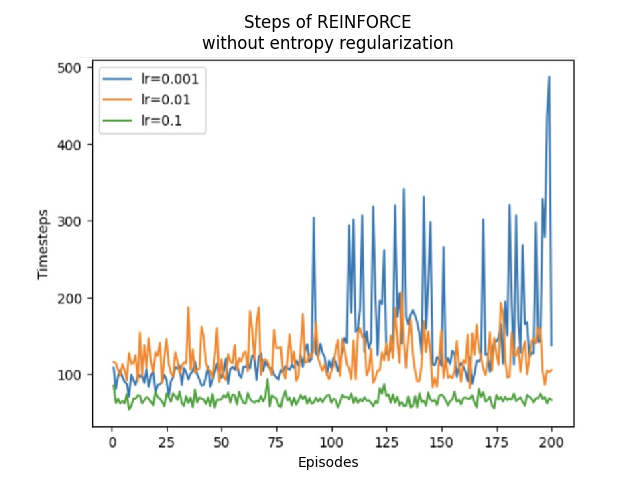
\includegraphics[width=0.85\linewidth]{Report/images/03.Steps_of_REINFORCE_without_ER.png}
\caption{\label{fig:ReinforceEntropy_Rewards}The figure above shows the steps of REINFORCE without entropy regularisation with different learning rates. As we can see, almost learning rates show a rising trend of steps, with the graph for learning rates 0.01 and 0.001 showing the most promise. }
\end{figure}
\par Figure 2 and 3 shows our results for REINFORCE without entropy regularisation. While REINFORCE is touted as a simpler Policy Gradient method it can often suffer from high variances causing slower convergence to optimal values because it requires an entire episode to be sampled. This is very visible from the results. Even after an average results of over 1000 episodes, we are unable to see a dramatic rise in learning as we expected. However, we can see the effect of learning rate on model performance as learning rates of 0.001 and 0.01 outperform learning rate of 0.1. 

\begin{figure}[h!]
\centering
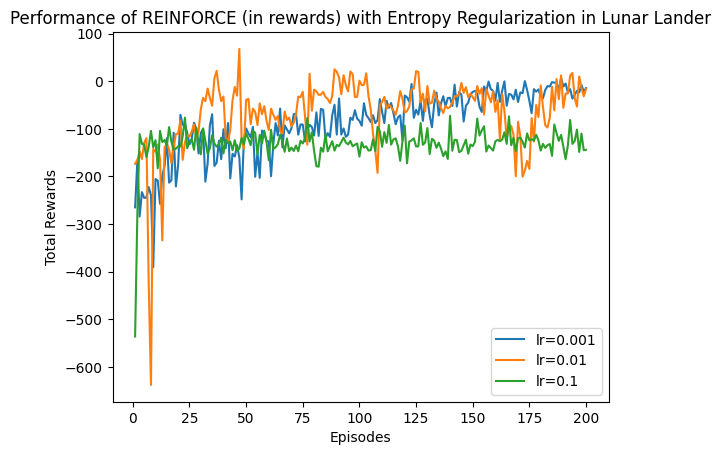
\includegraphics[width=0.85\linewidth]{Report/images/04.Performance_of_REINFORCE_with_ER_Rewards.png}
\caption{\label{fig:ReinforceEntropy_Rewards_LR}The figure above shows the rewards of REINFORCE with entropy regularisation with different learning rates. As we can see, all learning rates show a rising trend of rewards, with the graph for learning rates 0.01 and 0.001 showing the most improvement and the learning rate 0.1 stabilising but not showing much improvement. }
\end{figure}


\begin{figure}[h!]
\centering
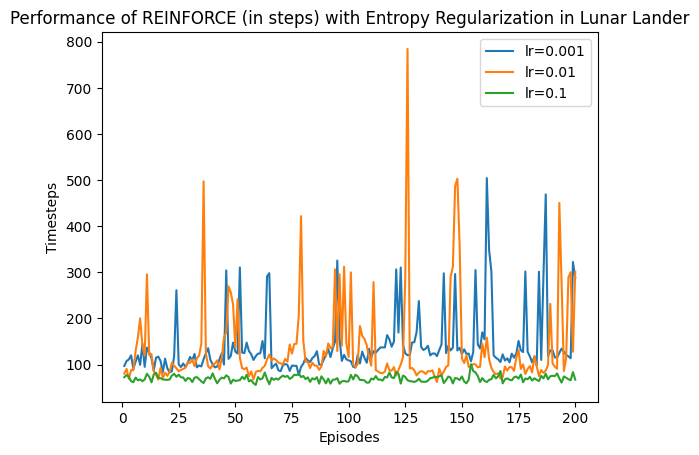
\includegraphics[width=0.85\linewidth]{Report/images/05.Performance_of_REINFORCE_with_ER_Steps.png}
\caption{\label{fig:ReinforceEntropy_Rewards_Steps}The figure above shows the total steps of REINFORCE with entropy regularisation with different learning rates. As we can see, all learning rates show a rising trend of rewards, with the graph for learning rates 0.01 and 0.001 showing the most improvement and the learning rate 0.1 stabilising but not showing much improvement. }
\end{figure}
\par To improve our existing results we decided to implement a version of REINFORCE that includes entropy regularisation and as seen from our figure 4, the learning is much better and a faster convergence as learning rates begin rising. This is because the inclusion of an entropy term to the loss function helps penalise trajectories with lesser randomness (or entropy) and thus encourages the policy network to explore more diverse state and action spaces, increasing exploration and preventing getting stuck in local maxima. 
  

\subsection{Actor-Critic Methods}
\par In the REINFORCE algorithm, we did not observe the fast convergence to optimal values as we hoped. This was probably because in REINFORCE algorithms, the entire episode must be sampled and thus suffers from high variance. In this section we will discuss Actor Critic methods, which provide a solution to combat high variance by combining the advantages of both value-based and policy-based methods and achieve optimal converging rewards. 
\par Actor Critic methods are Temporal Difference methods and have a separate memory structure to store the policy function independent of the value function. They generally have two neural networks: a policy structure known as an \emph{actor} and an estimated value function known as the \emph{critic}. While the policy function (or actor) returns a probability distribution of actions that can be taken in specific states, a value function (or the critic) determines the expected reward gained by following the policy. \cite{actor-critic}. Thus the value function is called a critic as it criticises the actions taken by the actor in the form of a TD error. This scalar signal indicates whether the actions taken by the agent are better or worse than what the critic expected. 
\par The TD error can be evaluated as follows in the following equation
\begin{equation*}
\delta_{t} = R_{t+1} + \gamma * V_t(S_{t+1})-V_t(S_t)
\end{equation*}
 where 
\begin{itemize}[itemsep=0.0pt]
\renewcommand\labelitemi{.}
\item $\delta_{t}$ is the temporal difference error at timestep $t$
\item $R_{t+1}$ is the reward for transitioning from state $S_t$ to the state $S_{t+1}$
\item $\gamma$ is the discount factor which discounts future rewards
\item $V_t(S_{t+1})$ is the estimated value of going to state $S_{t+1}$ at timestep t according to the critic. This represents the estimated cumulative rewards that can be gained from step $S_{t+1}$ onwards.
\item $V_t(S_t)$ is the estimated value of going to state $S_t$ according to the critic. This represents the estimated total rewards that can be gained from step $S_{t}$ onwards.
\end{itemize}

Thus, a positive TD error ($\delta_{t}$ \textgreater 0) indicates that the value of transitioning from state $S_t$ to $S_{t+1}$ is greater than expected and thus the action responsible should be taken more often. On the other hand a negative TD error ($\delta_{t}$ \textless 0) indicates that the value of transitioning from state $S_t$ to $S_{t+1}$ is lesser than expected and thus the action responsible should be avoided in the future. Thus, through this iterative process of updating the TD error the Actor Critic algorithm tends to strike a balance between exploration and exploitation. The actor explores the state space and taking more diverse actions and the critic evaluating the consequences of the actions. When the actions are more risky and produce lesser expected returns the TD error is negative and when they are more fruitful and produce higher expected returns the TD error is positive.

\subsubsection{Bootstrapping}
%\par A variation of Actor-Critic incorporates a bootstrapping technique. In the REINFORCE algorithm, because the entire episode must be sampled, its variance is high. The Actor Critic method combines value-based and policy-based methods, achieving both low variance and low bias. The Actor Critic method incorporates the bootstrapping technique to improve estimates of cumulative rewards. By using bootstrapping, the Actor Critic method can use the Critic's immediate feedback to adjust the Actor's strategy, thus achieving a better balance between exploring the environment and learning optimized action strategies.. 
\par A variation of Actor-Critic incorporates a bootstrapping technique which combines elements of both policy-based and value-based methods. In this architecture the actor, as usual, learns a parameterized policy function $\pi_\theta$ that maps states to actions. The critic uses bootstrapping to update the value function and estimate the value of the state-action pairs. Thus, instead of waiting for the cumulative rewards from the environment it updates the value function using its own estimates. By using bootstrapping, the Actor Critic method can use the Critic's immediate feedback to adjust the Actor's strategy, thus achieving a better balance between exploring the environment and learning optimized action strategies.
The descent advantage loss allows the actor to choose the actions that outperform the baseline by minimising the difference between them, while the ascent policy gradient drives policy updates to maximize the cumulative reward by increasing the likelihood of selecting actions with higher advantages.

The algorithm for Actor-Critic with Bootstrapping is given below \cite{plaat-deeprl}
\begin{algorithm}[h!]
\caption{Actor-Critic with Bootstrapping}
\SetAlgoLined
\DontPrintSemicolon
\small % Set font size to small
\KwData{parameter $\theta$, policy function $\pi_\theta$, maximum timesteps $T$, number of episodes $E$, estimation depth $n$, learning rate $\alpha$, value function $V_\phi (s)$}
Initialise $\theta$ and $\phi$ arbitrarily\;\\
\item \textbf{Repeat} \;\\
\For{$e \in 1$ \KwTo $E$}
{
    \item Initialise state $s$\;
    \item Sample trajectory $\tau$ = ${s_0,a_0,r_1,....,s_T}$ for $\pi_\theta(a|s)$
     \item 
    \For{$t = 1$ \KwTo $T-1$}
    {
     \item Compute cumulative reward $\hat{Q}_n(s_t,a_t)$ for the n-step target
     \newline \(\hat{Q}^(s_t,a_t) = \sum_{k=0}^{n-1}\gamma^k\cdot r_{t+k} + \gamma^{n} \cdot V_\phi (s_{t+n})\)
    }
}
    \item $\phi \leftarrow \phi - \alpha \cdot \nabla_\phi \sum_t (\hat{Q}_n(s_t, a_t) - V_\phi(s_t))^2$ \;
    \item $\theta \leftarrow \theta + \alpha \sum_t [\hat{Q}_n(s_t, a_t) \nabla_\theta \log \pi_\theta(a_t | s_t)]$\;
\item \textbf{Until} $\nabla_\theta J(\theta)$ converges below $\epsilon$ \;
\item \textbf{Return} parameter $\theta$
\end{algorithm}

\par Figures 6, 7 and 8 show us the performances of Actor-Critic with bootstrapping when varying different hyper-parameters such as learning rate, the number of hidden layers and the number of neurons. As seen in figure 6 learning rate of 0.005 shows a jump in average returns compared to other learning rates. Furthermore, we can also see in figure 7 that bootstrapping with 2 or 3 hidden layers tends to learn faster than bootstrapping with only one hidden layer. Lastly, figure 8 shows the effects of the number of neurons on learning rate. We can see that neural networks with 64 neurons learn faster than neural networks with 128 or 256 neurons. While the results do provide some key insights, it is important to note that when averaging rewards in highly stochastic environments can lead to final graphs where the overall increase is not as dramatic.

\begin{figure}[h!]
    \centering
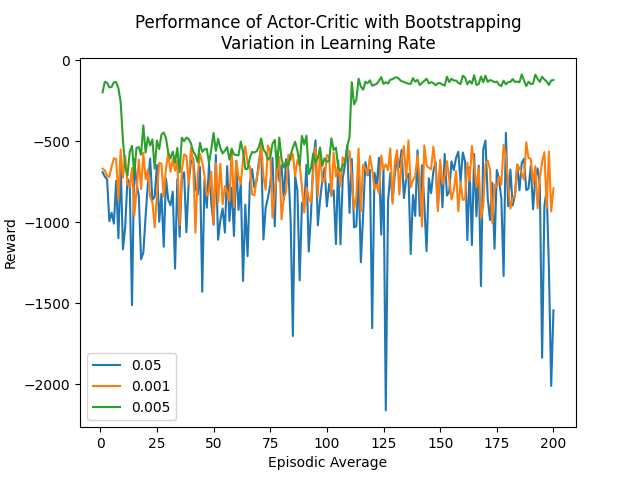
\includegraphics[width=0.85\linewidth]{Report/images/06.Performance_of_Actor_Critic_BS_LR.png}
\caption{\label{fig:ActorCritic for different learning rates}The figure shows the performance of Actor Critic with bootstrapping while varying learning rates. When the learning rate is set to 0.005, relatively good results are achieved in training the agent. However, after 1000 episodes (averaged over every 5 episodes for a total of 200 averages), the reward still remains below zero. Conversely, when the learning rate is set to a higher value (0.05) or a lower value (0.001), the agent does not train at all.}
\end{figure}

\begin{figure}[h!]
\centering
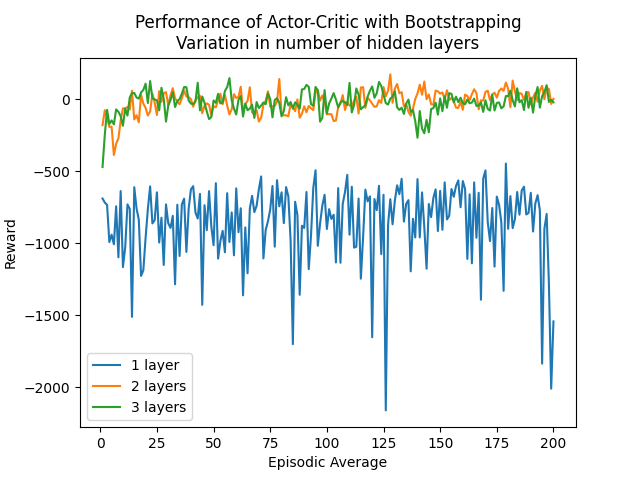
\includegraphics[width=0.85\linewidth]{Report/images/07.Performance_of_Actor_Critic_BS_Layers.png}
\caption{\label{fig:ActorCritic for different Hidden Layers}The figure shows the performance of Actor Critic with bootstrapping while varying the number of hidden layers. When both the policy network and the value network have only one hidden layer, the agent cannot be trained, as evidently seen in the graph. Increasing the hidden layers of these two networks can improve the training effect. The graph demonstrates the improvement in performance with more than one hidden layer, with a significantly better reward than with one hidden layer}
\end{figure}


\begin{figure}[h!]
\centering
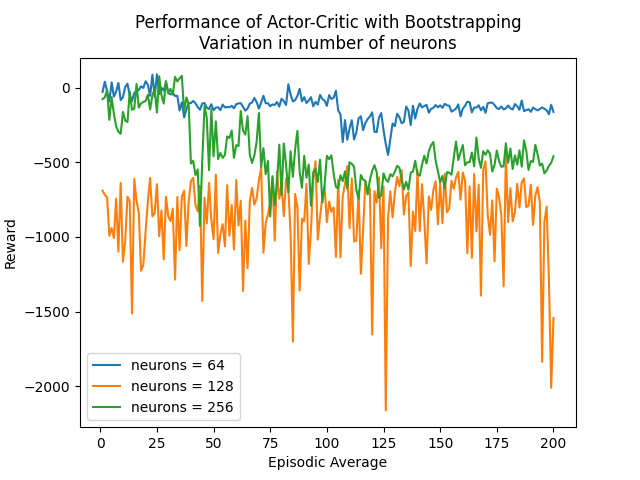
\includegraphics[width=0.85\linewidth]{Report/images/08.Performance_of_Actor_Critic_BS_Neurons.png}
\caption{\label{fig:ActorCritic for different Neurons}The result of Actor Critic with different neurons. According to results of different network layers, we set both the policy network and the value network to have two hidden layers. The results shows that networks with fewer neurons tend to perform relatively better, but there is still a long way to go before the agent is successfully trained.}
\end{figure}

\subsubsection{Baseline Subtraction}
Actor-Critic algorithms could also employ baseline subtraction which is a technique used to reduce the variance and improve convergence. We recall the previous policy gradient function denoted by 

\begin{equation*}
\nabla_\theta J(\theta) = \mathbb{E}_\pi[\sum _{t=0}^{T-1}  \nabla_\theta \log\pi_\theta (a_t|s_t)G_t]
\end{equation*}

By subtracting a baseline $b(s_t)$, typically a value function,  from the observed cumulative reward helps reduce make them smaller and more stable. This reduces the variance, without changing the expectation. \cite{david-ucl-lecture}

The updated policy gradient function after baseline subtraction is shown below. 

\begin{equation*}
\nabla_\theta J(\theta) = \mathbb{E}_\pi[\sum _{t=0}^{T-1}  \nabla_\theta\log\pi_\theta (a_t|s_t)G_t - b(s_t)]
\end{equation*}
\begin{algorithm}[h!]
\caption{Actor-Critic with Baseline Subtraction}
\SetAlgoLined
\DontPrintSemicolon
\small % Set font size to small
\KwData{parameter $\theta$, policy function $\pi_\theta$, maximum timesteps $T$, number of episodes $E$, estimation depth $n$, learning rate $\alpha$, value function $V_\phi (s)$}
\KwResult{Selected action}
Initialise $\theta$ and $\phi$ arbitrarily\;\\
\For{$e = 1$ \KwTo $E$}
{
    Initialise state $s$\;
     \item Sample trajectory $\tau$ for $\pi_\theta$
     \item
    \For{$t = 1$ \KwTo $T-1$}
    {
     \item Compute advantage function using the cumulative reward and the value function;
     \(\hat{A}_n(s_t,a_t) = \hat{Q}_n(s_t,a_t) - V_\phi(s_t)\)
    }
    \item Compute descent advantage loss $\phi$
    \item Compute ascent policy gradient $\theta$
}
\State \Return parameter $\theta$
\end{algorithm}
\begin{figure}[h!]
\centering
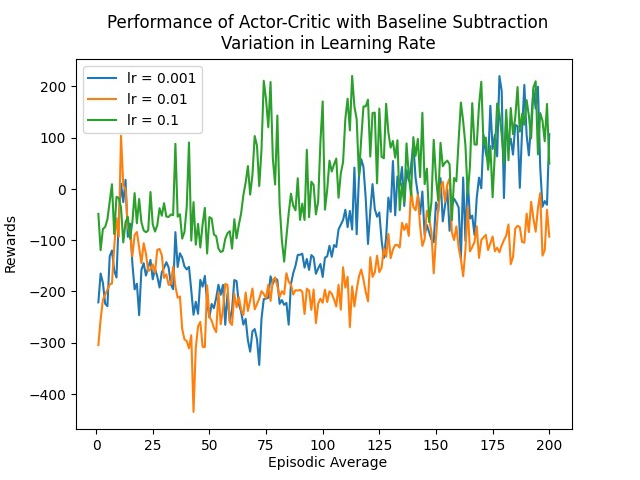
\includegraphics[width=0.85\linewidth]{Report/images/09.Performance_of_Actor_Critc_BSub_LR.png}
\caption{\label{fig:ActorCritic with Baseline Subtraction - Variation in Learning Rate}The result of Actor Critic with Baseline Subtraction with different learning rates. 
When evaluating three different learning rates (0.001, 0.01, 0.1), it was observed that the rate of 0.1 achieved the highest reward after averaging across 200 episodes. The learning rate of 0.001 initially shows slow progress but gradually improves over time. On the other hand, the learning rate of 0.01 results in the poorest performance.}
\end{figure}

\begin{figure}[h!]
\centering
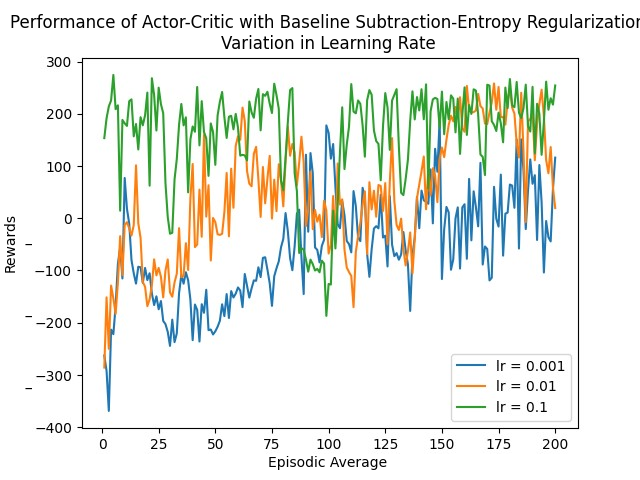
\includegraphics[width=0.85\linewidth]{Report/images/13.Performance_of_Actor_Critc_BSubandER_LR.png}
\caption{\label{fig:ActorCritic with Baseline Subtraction and Entropy Regularization - Variation in Learning Rate}The result of Actor Critic with Baseline Subtraction and entropy regularization with different learning rates. 
When evaluating three different learning rates (0.001, 0.01, 0.1), it was observed that the rate of 0.1 achieved the highest reward after averaging across 200 episodes. The learning rate of 0.001 initially shows slow progress but gradually improves over time. On the other hand, the learning rate of 0.01 results in the poorest performance.}
\end{figure}
Figure 9 and Figure 10 compares the performances of Actor-Critic with Baseline Subtraction, with and without entropy regularization. Both agents were tested against learning rates of 0.001, 0.01 and 0.1. As seen from figure 9, the algorithm provided better returns than vanilla Actor-Critic algorithms. However, the rewards were lower than that of entropy regularization. In figure 10, it is evident that the returns are more (comparing the rewards of a learning rate of 0.1). However, a low learning rate such as 0.001 is not beneficial, as the gain is much slower than a learning rate of 0.1. 
\subsubsection{Bootstrapping and Baseline Subtraction}
Certain Actor-Critic algorithms combine both bootstrapping and baseline subtraction. They combine the advantages of bootstrapping by using the Critic's feedback to adjust the Actor's strategy and by using baseline subtraction to reduce the variance and keep the rewards small, while maintaining stability. This is achieved by using both descent advantage loss and ascent policy gradient.  
The equations for Descent Advantage Loss and Ascent Policy Gradient are given below. 
\par Descent Advantage Loss is calculated by 
\begin{equation*}
\theta \leftarrow \theta - \alpha * \nabla_\theta\Sigma_t(\hat{A}_n(s_t,a_t))^2
\end{equation*}
Ascent Policy Gradient is calculated by 
\begin{equation*}
\theta \leftarrow \theta + \alpha * \Sigma_t[\hat{A}_n(s_t,a_t)*\nabla_\theta\log\pi_\theta(a_t|s_t)]
\end{equation*}

Where 
\begin{itemize}[itemsep=0.0pt]
\renewcommand\labelitemi{.}
\item $\theta$ is the parameter of the policy function
\item $\alpha$ is the learning rate
\item $\gamma$ is the discount factor which discounts future rewards
\item $\hat{A}_n(s_t,a_t)$ is the advantage function which represents the estimated advantage of taking an action $a_t$ in the state $s_t$
\item $\nabla_\theta$ represents the gradient with respect to the policy parameters $\theta$
\end{itemize}
Both descent advantage loss and ascent policy gradient uses the advantage function. The advantage function subtracts the value V from a state-action value estimate Q. This allows to estimate how better the action is, compared to the expectation at that state. This is expressed as 
\begin{equation*}
    \hat{A}_n(s_t,a_t) = \hat{Q}_n(s_t,a_t) - V_\phi(s_t)
\end{equation*}
to estimate the cumulative reward \(\)
\begin{algorithm}[h!]
\caption{Actor-Critic with Bootstrapping and Baseline Subtraction}
\SetAlgoLined
\DontPrintSemicolon
\small % Set font size to small
\KwData{parameter $\theta$, policy function $\pi_\theta$, maximum timesteps $T$, number of episodes $E$, estimation depth $n$, learning rate $\alpha$, value function $V_\phi (s)$}
\KwResult{Selected action}
Initialise $\theta$ and $\phi$ arbitrarily\;\\
\For{$e = 1$ \KwTo $E$}
{
    Initialise state $s$\;
     \item Sample trajectory $\tau$ for $\pi_\theta$
     \item
    \For{$t = 1$ \KwTo $T-1$}
    {
     \item Compute cumulative reward $\hat{Q}_n(s_t,a_t)$  for the n-step target
     \item Compute advantage function using the cumulative reward and the value function;
     \(\hat{A}_n(s_t,a_t) = \hat{Q}_n(s_t,a_t) - V_\phi(s_t)\)
    }
    \item Compute Descent Advantage Loss $\phi$
    %\newline
     %\(\phi \leftarrow \phi - \alpha \cdot \nabla_\theta\Sigma_t(\hat{A}_n(s_t,a_t))^2\) 
     \item Compute Ascent Policy Gradient $\theta$
     %\newline 
    %\(\theta \leftarrow \theta + \alpha \cdot \Sigma_t[\hat{A}_n(s_t,a_t)*\nabla_\theta\log\pi_\theta(a_t|s_t)]\)
}
\State \Return parameter $\theta$
\end{algorithm}
\begin{figure}[h!]
\centering
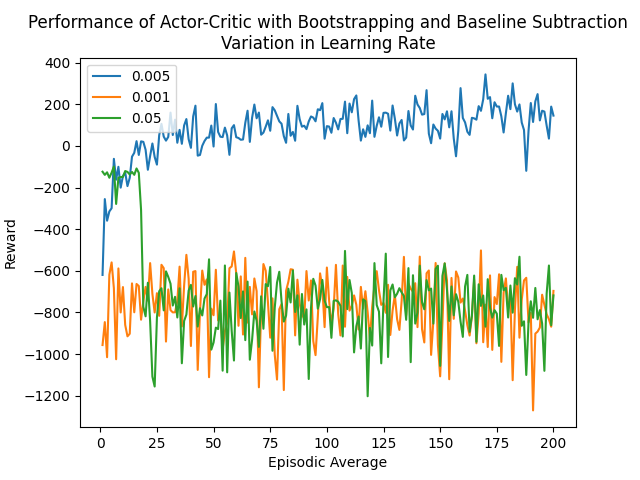
\includegraphics[width=0.85\linewidth]{Report/images/10.Performance_of_Actor_Critic_BSandBS_LR.png}
\caption{\label{fig:ActorCriticBS2-different learning rates}The figure above shows the rewards of Actor Critic with Bootstrapping and Baseline Subtraction with different learning rates. The results were averaged over every 5 episodes. As seen in the graph, the learning rate of 0.005 show a rising trend in rewards when compared to a learning rate of 0.001 and 0.05}
\end{figure}

\begin{figure}[h!]
\centering
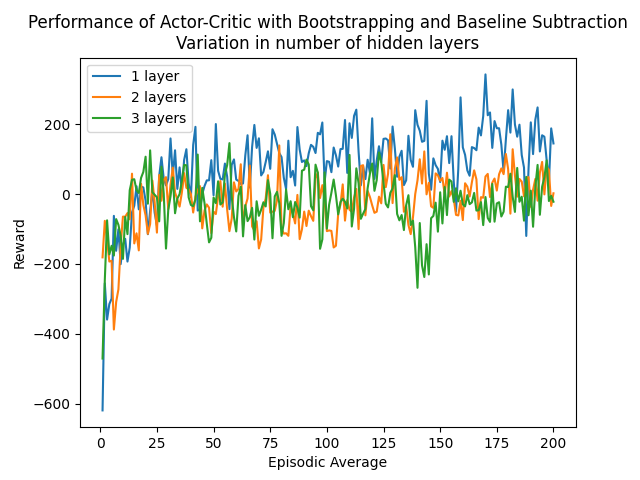
\includegraphics[width=0.85\linewidth]{Report/images/11.Performance_of_Actor_Critic_BSandBS_Layers.png}
\caption{\label{fig:ActorCriticBS2-different neurons}The results of Actor-Critic with Bootstrapping and Baseline Subtraction with variations in number of hidden layers of the policy network and the value network. The results were averaged over 2 episodes. The graph shows comparable performance with 1, 2 and 3 hidden layers, with 1 hidden layer performing slightly better than 2 and 3 hidden layers. }
\end{figure}

\begin{figure}[h!]
\centering
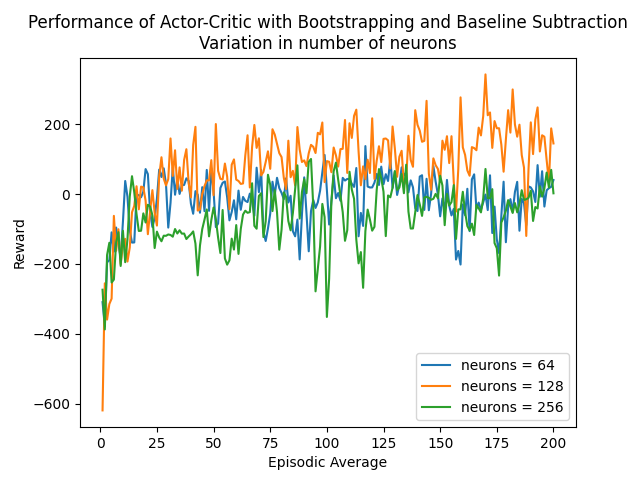
\includegraphics[width=0.85\linewidth]{Report/images/12.Performance_of_Actor_Critic_BSandBS_Neurons.png}
\caption{\label{fig:ActorCriticBS2-different hidden layers}The results of Actor-Critic with Bootstrapping and Baseline Subtraction with variations in number of neurons of the policy network and the value network. The results show that the layers with 128 neurons provided better results, when compared to layers with 64 neurons and 256 neurons. When the number of neurons was set to 128, the agent achieved a better reward, reaching a peak value of over 200. In comparison, networks with 64 and 256 neurons achieved slightly poorer training results.}
\end{figure}
Figures 11, 12 and 13 shows the performances of Actor-Critic with Bootstrapping and Baseline Subtraction when various hyper-parameters are tuned such as learning rate, number of hidden layers and number of neurons. 
As seen in Figure 11,  a learning rate of 0.1 provides better results when compared to learning rates of 0.001 and 0.01. The learning rate of 0.001 shows slower progress, but improves gradually. From figure 12, it is observed that the number of hidden layers did not play a significant role, surprisingly. All 3 variations performed similarly, with a variation of 1 and 2 hidden layers performing slightly better. The performance of Actor-Critic agents with bootstrapping and baseline subtraction was graphed out in Figure 13. Here, it is seen that 128 is the optimal number, with a steep improvement in performance, as it produced better results, when compared to 64 and 256 neurons. 
\section{Goals Achieved}
\subsection{Effects of Policy Gradients of REINFORCE on Variance}
\par As we can see from the results of our implementation of REINFORCE, Policy Gradient methods can have a de-stabilising effect on rewards, particularly in high-dimensional state spaces such as Lunar Lander. We can see this with the high amount of noise generated in our average reward and time step plots in figures 2 and 3. This may be because REINFORCE samples entire trajectories (series of states, actions and rewards) stochastically rather than observing the rewards gained from individual states or actions and thus there can be high variability in the returns produced by different trajectories which may only be differ by one action or state. Furthermore, since this environment is more complex than classical environments like CartPole, the probability distribution produced can have a high variance between different state% Policy graThey do this by providing an output of  probability distribution over actions in a certain state and by optimising the stochastic policy function such that actions with more than expected returns are more likely than actions with less than expected returns. This is different from value-based methods that store the value of each state-action pair and select a single deterministic action that is suitable at any state the agent is in.  
\par We can see that the implementation of Entropy Regularisation in REINFORCE helps to significantly reduce noise in REINFORCE. This can be seen by the difference in noise in Figure 2 and 4. This is because Entropy Regularisation can help the architecture balance the exploration-to-exploitation ratio, allowing the agent to explore more unfamiliar state spaces in some cases and prioritizing greedy actions in others.
\subsection{Effects of Bootstrapping and Baseline Subtraction On Policy Gradients}
\par  While bootstrapping is done to reduce the variance of the policy gradient, we observe that bootstrapping itself is not sufficient to help the architecture achieve rewards that converge to a stable optima over time. This is evident from our results in figure 6, 7 and 8. This may be because while bootstrapping tries to bring the advantages of value-based learning to policy-based learning, it may end up doing the exact opposite in the form of higher instability when value estimates are updated based on unstable environment rewards by the critic. This often causes the instability to explode and propagate further. However, bootstrapping combined with baseline subtraction works much better than bootstrapping alone. This is shown by our positive results in 10, 11 and 12. This is because the subtraction of a baseline term from estimated advantages helps to compensate for the variance generated by bootstrapping, allowing the estimated advantages to be more stable and accurate, allowing faster convergence.
\subsection{Comparison of Performance}
\par First, we compared the results of the REINFORCE algorithm. When we used REINFORCE without entropy regularization, we tested three different learning rate settings, and it turns out that the smallest value (0.001) achieved the best results. However, when entropy regularization was added to the model, none of the three learning rates achieved equally good results.
\par For the Actor-Critic model, the results indicate that using only the bootstrapping technique does not lead to ideal outcomes. Employing only baseline subtraction can result in relatively more satisfactory rewards, but the best approach is to combine these two techniques, which can push the final reward to exceed 200.
Comparing the best outcomes of REINFORCE and Actor-Critic clearly demonstrates the superiority of the Actor-Critic algorithm in our study.
\subsection{Effect of entropy regularization on performance}
\par As explained earlier, entropy regularization promotes action diversity. This is evidently seen in Figure 2 and Figure 4 for REINFORCE agent, particularly with a learning rate of 0.01. The REINFORCE agent with entropy regularization provides higher rewards, when compared to the agent without regularization. This is also seen in Figure 9 and Figure 10, actor-critic with baseline subtraction. The actor-critic agents with entropy regularization performed better with learning rates 0.01 and 0.1, than without entropy regularization. The rewards were consistently higher and the curve was more stable. This shows that entropy regularization influences policy optimization and stability of the agents.
\bibliography{Report/references}
\bibliographystyle{Report/reference_style}
\end{document}